\documentclass{standalone}
\usepackage{tikz}
\usetikzlibrary{backgrounds}

% Define custom colors and styles
\definecolor{eulerblue}{RGB}{0, 102, 204} % Dark blue for Eulerian sources
\definecolor{lagrangianred}{RGB}{255, 102, 102} % Light red for Lagrangian sources
\definecolor{broadorange}{RGB}{255, 165, 0} % Orange for Broad sources

\tikzset{
    eulerline/.style={draw=eulerblue, fill=eulerblue!50, opacity=0.5},
    lagrangianline/.style={draw=lagrangianred, fill=lagrangianred!50, opacity=0.5},
    broadline/.style={draw=broadorange, fill=broadorange!50, opacity=0.5},
}

\begin{document}
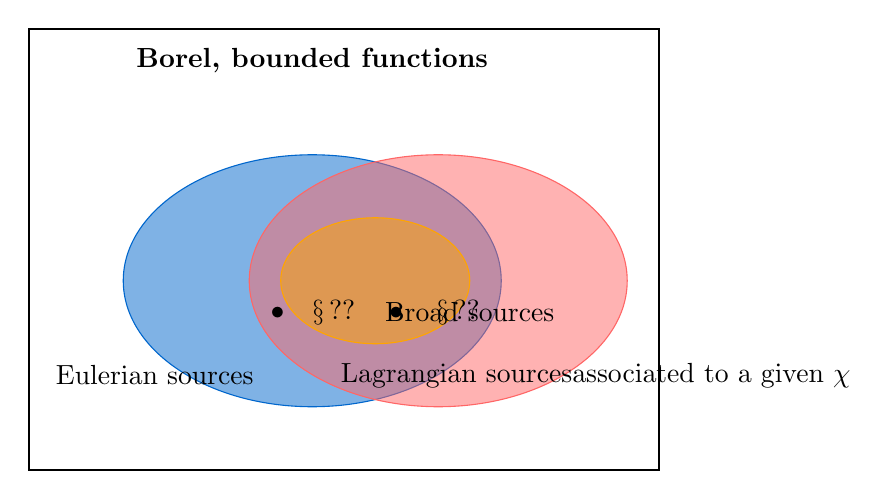
\begin{tikzpicture}[scale=0.8]
    % Title
    \node at (0,3.5) {\textbf{Borel, bounded functions}};
    
    % Eulerian sources ellipse
    \fill[eulerblue, fill opacity=0.5] (0,0) ellipse (3 and 2);
    \draw[eulerblue] (0,0) ellipse (3 and 2);
    \node at (-2.5, -1.5) {Eulerian sources};
    
    % Lagrangian sources ellipse
    \fill[lagrangianred, fill opacity=0.5] (2,0) ellipse (3 and 2);
    \draw[lagrangianred] (2,0) ellipse (3 and 2);
    \node at (4.5, -1.5) {Lagrangian sources\\associated to a given $\chi$};
    
    % Intersection area (Broad sources)
    \fill[broadorange, fill opacity=0.5] (1,0) ellipse (1.5 and 1);
    \draw[broadorange] (1,0) ellipse (1.5 and 1);
    \node at (2.5, -0.5) {Broad sources};
    
    % Central labels
    \node at (1, -0.5) {$\bullet \quad \mathsection \, ?? \quad \bullet \quad \mathsection \, ??$};
    
    % Frame around the diagram
    \draw[thick] (-4.5, 4) rectangle (5.5, -3);
\end{tikzpicture}
\end{document}